% 固定源第16题：等腰梯形水渠与虚线抛物线，几何示意
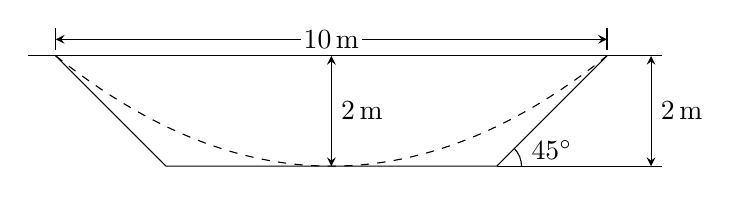
\begin{tikzpicture}[scale=0.7,>=stealth]
  \draw (-5,2)--(-3,0)--(3,0)--(5,2);
  \draw (-5.5,2)--(5.5,2);
  \draw[dashed,domain=-5:5,samples=100] plot (\x,{0.08*\x*\x});
  \draw[<->] (-5,2.3)--(5,2.3) node[midway,fill=white,inner sep=1pt] {$10\,\mathrm{m}$};
  \draw (-5,2.1)--(-5,2.5) (5,2.1)--(5,2.5);
  \draw[<->] (0,0)--(0,2) node[midway,right] {$2\,\mathrm{m}$};
  \draw[<->] (5.8,0)--(5.8,2) node[midway,right] {$2\,\mathrm{m}$};
  \draw (3,0)--(6,0) (5,2)--(6,2);
  \draw (3.45,0) arc (0:45:0.45);
  \node at (4.0,0.30) {$45^\circ$};
\end{tikzpicture}
